\section{Defining the Structure}
\begin{figure}
    \centering
        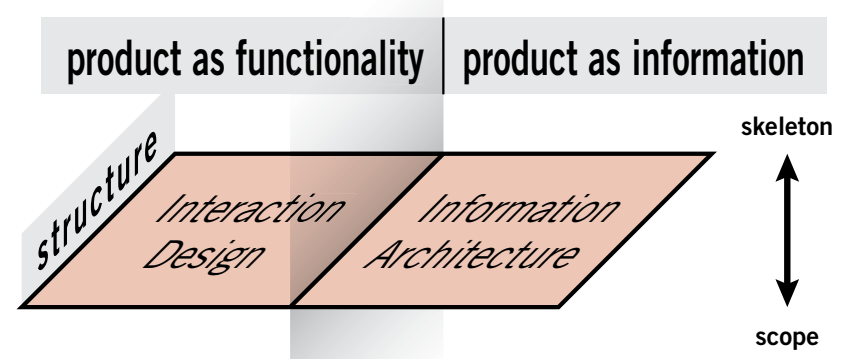
\includegraphics[width=12cm]{images/pic6.png}    
    \caption{}
\end{figure}
common between interaction design and information architecture: defining patterns and sequences in which options will be presented to user.
Information architecture deals with options involved in conveying information to user.
\section{Interaction Design}
Describes possible user behaviour and How the system will respond. Like a dance together.
\subsection{Conceptual Models}
Users' impressions of how the interactive components we create will behave are known as conceptual models.
\subsection{Error Handling}
What does the system do when people make mistake and what can the system do to prevent that.
\section{Information Architecture}
We should structure information, so that other people can use it. 
\subsection{Structuring Content}
To create organizational and navigational schemes that allow users to move through site content efficiently and effectively. It is related to the field of information retrieval(the
 design of systems that enable users to find information easily). \\
 We have to approaches:
 \begin{itemize}
     \item \textbf{top-down approach: } to start with the broadest category of possible content and 
     then we break it down into subcategories
     \item \textbf{bottom-up approach: }
 \end{itemize}
\subsection{Architectural Approaches}
The term \textbf{node} may refer to page, document and component. In a hierarchical structure, nodes have parent/child relationships with othe nodes. 
\begin{figure}[]
    \centering
        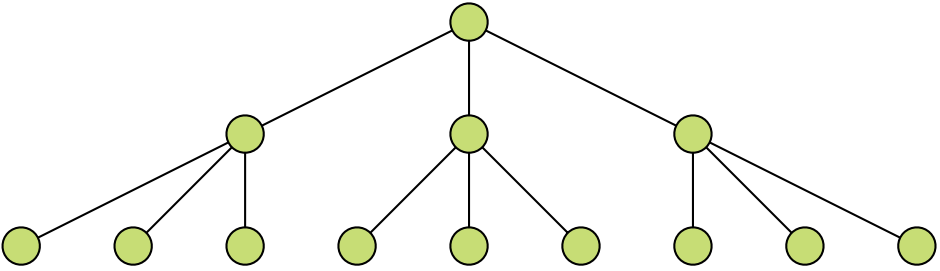
\includegraphics[width=12cm]{images/pic7.png}    
    \caption{Hierarchical structure}
\end{figure}
\subsection{Organizing Principles}
\subsection{Language and Metadata}
\section{Team Roles and Process}